% SECTION 
% 	A neural coarse graining theory of consciousness

\rlstart{5}

        In this section, we propose a new theoretical framework of consciousness \{\tnamefull\}\todo{We need a good name}. This framework proposes that NTIC is the fundamental property for information processing to be conscious. Additionally, coarse-graining is necessary to achieve NTIC in various of different systems. 

        We starts our argument from the first presumptive fact that every human conscious precept is highly informative. Our conscious experience always consists of high multidimensional information and usually involves information from multiple modalities. The notion of information referred to in this article is considered as resolved uncertainty. Being a certain conscious state rules out other enormous possible conscious experience in the state space of conscious experience. Therefore, every conscious percept resolves a huge amount of uncertainty and provides considerable information. 
        
        This notion is in agreement with one of the axiom, \textit{information}, in Integrated Information Theory (IIT 3.0) which claims that \myQuote{...an experience of pure darkness is what it is by differing, in its particular way, from an immense number of other possible experiences...} \citep[p. 2]{oizumi2014phenomenology}.
        
        Based on this presumptive fact, we postulate that the amount of information possessed of a conscious percept should be equivalent to information involved in a particular event or entity in the physical reality. Strictly speaking, we recognise information is a common language between conscious experience and the physical reality. We further take a radical standpoint and postulate that consciousness is fundamentally associated with information, i.e. information correlates of consciousness (ICC), \cite{chalmers1996conscious, tononi2004information, gamez2011information, Gamez2016}) and discard the notion of neural correlates of consciousness(NCC). 
        
        Next, we next consider the second presumptive fact that the information in consciousness is bound. Even though information involved in every conscious percept is extremely rich, it is still limited and we do not consciously feel everything in this universe. This leads to the boundary problems of consciousness \cite{goff2006experiences}. There should exist information boundaries for every conscious entity. Presuming consciousness is information-based phenomenon, we can identify the boundaries with measures from information theory. Particularly, in this case, boundaries can be defined by information closure. Therefore, information closure should be observed in conscious entities in the physical reality. 
        
        
        \rewording{informational closure also suggests that there is no information flow from the lower to the higher level. Knowledge of the microscopic levels will not improve predictions of the future states of the macroscopic levels \citep{PFANTE.2014}}. 
        Information closure also implies that the system is ignorant of information outside of the system. Therefore, if a coarse-grained level achieves information closure, it suggests the NTIC process at the coarse-grained level is ignorant of information processing happening at microscopic levels and also higher coarse-grained levels. This virtually makes the informational closed macroscopic levels as a complete reality. 
        \todo{Due to my concern mentioned last week, I think I should also mention the closure is not only to the environment but also to the microscopic levels}
        
        Finally, our conscious experience always reflects some degree of information about environment and bodily states, i.e. non-trivial information. To account for the information-based considerations, we propose that NTIC is a fundamental informational property associated with consciousness. 
        
        
        
        \begin{WritingMaterials}
        For example, considering two physical systems (Alice and Bob) and there is no interaction (or information passing) in between. Assuming that Alice is conscious, the conscious experience that Alice has should not involve any information about Bob. 
        
        \todo{Considering putting this para}
        Similarly, we can apply this scenario to brain processing between two regions. We can consider a thought experiment. 
        Imagining that in the future, one poor subject attend this experiment. We remove the subject's visual cortex from other brain areas. However, we keep all the connection between the two parts of the brain intact by replacing dendrites and axons between the two parts with micro electronic cables. Because these cables are very long, we can move the visual cortex to the surface of Mars. Now the experimenters give visual cortex a input signal. If the signal travels with the speed of light, it still takes three seconds to reach the other part on the earth. We can ask: Between the experimenters send the input signal and the information reach the part on the earth, what visual conscious content does the subject experience in the three seconds? We presume that in this three seconds subject's conscious experience should not contain any information about the visual input. Otherwise, the subject may be able to use the information to perform subsequent actions. This violates physics. This may look like a trivial questions.
        

        However, in many systems, it is difficult to achieve NTIC at microscopic levels due to stochasticity. Through coarse-graining, NTIC processes become possible at macroscopic levels. Therefore, coarse-graining is necessary for many biological systems to implement NTIC processes, especially for the neural system (Fig. \ref{fig:LevelOfConsciousness}). In the following, we explained this framework and provide mathematical definitions and implications of ICC.  
        \end{WritingMaterials}
        

		\begin{WritingMaterials}
		
        @ As we mentioned in Chapter 3, to form non-trivial informational closure has a huge evolutionary advantage for the creatures interacting with the environment at our scale. 
        
        @ The physical environment dynamic at the human scale are nearly deterministic.\needref{Do we need ref here?}
        
		@ To maximise fitness for individual human-being, neural system should try hard to infer and model the deterministic physical rules.

		@ This drives the neural system to create a non-trivial informational closure.
		
        @ Therefore, NTIC emerges from evolutionary processes is functionally plausible. 
        
        @ Importantly, at the microscopic level, it is impossible to achieve NTIC as we mentioned in chapter 2.

		@ However, at a macroscopic scale, information processing can achieve non-trivial informational closure (Fig. \ref{fig:LevelOfConsciousness})
        
        @ Therefore, the NTIC correlating conscious experience must settled at coarse-grained macroscopic levels.
        
		@ Through coarse-graining, we can define a new set of variables.

        @ information is scale-dependent
        
		@ If the new set of variables are informational closure, then this creates a new \textit{reality} for all the variables inside.        
		@ \textit{Reality} here means that the all the future states of the system are driven by the current information (include variables and the relationships) within the boundary. 
			
        @
        
        @ Relationship between coarse-graining, scale and interaction with environment
        
        
		@ \rewrite{
			This illustrates how coarse-graining allows the formulation of incomplete generalizations that are relatively invariant, although at the cost of predictive precision regarding fine-grained details.} \cite{price2007causation}

			@@ conscious perception are very stable and time invariant.
			@@ Conscious perception is informative but we loss all the precise information about the states at microscopic level.        
        
        @ To summaries, in our framework, consciousness is 
			    @@ Intrinsic 
			    
			    @@ Informative  
			    
				@@ scale-dependent 

        % our claim   
			@ We claim that the state of a coarse-grained scale which realises non-trivial informational closured correlates the state of consciousness.

			@ We further postulate that level of consciousness corresponds to informational closureness of processes.

			@ The contents of consciousness correspond to the states of the non-trivial informational closure.

				
		% Following
			@ In the following part, we....\todo{todo}


			@ This is the same as "if a tree falls in a forest" thought experiment.

			@ Therefore, to understand this system, you don't need more information from external environment.

			@ It also means everything in this system is self-defined.
			
			
			@ \critical{I need to somehow acknowledge \cite{pennartz2017consciousness}}
				@@ \rewrite{ In conclusion, for a well-behaved representational system, it does not matter whether a neural activation pattern represents an external world feature truthfully or not, as long as the system represents the feature consistently over time and in sensory space.}

				@@ pennartz levels are defined by functional elements call "functional ensembles". \cite{pennartz2017consciousness} \rewrite{This delineation is different from a scale-based distinction of levels, because different levels are distinguished here based on function , i.e., what each level can accomplish in terms of computation and representation, culminating in perception at the highest level.}

			@ \rewrite{
				Multilevel views on consciousness and cognition have been expressed before by many other theorists, such as Oppenheim and Putnam (1958), Attneave (1961), Hofstadter (1979, 1985), Churchland and Sejnowski (1992), Wimsatt (1994), and Lycan (1996).} \cite{pennartz2017consciousness}
                
				@@ Oppenheim , P. , \& Putnam , H. ( 1958 ). Unity of science as a working hypothesis . In H. Feigl , G. Maxwell , \& M. Scriven (Eds.), Concepts, theories, and the mind – body problem (pp. 3 – 36 ). Minneapolis : University of Minnesota Press .
				@@ Attneave , F. ( 1961 ). In defense of homunculi . In W. A. Rosenblith (Ed.), Sensory communication (pp. 777 – 782 ). Cambridge, MA : MIT Press .
				@@ Hofstadter , D. R. ( 1979 ). Godel, Escher, Bach, an eternal golden braid . New York : Basic Books .
				@@ Churchland , P. S. , \& Sejnowski , T. J. ( 1992 ). The computational brain . Cambridge, MA : MIT Press .
				@@ Wimsatt , W. C. ( 1994 ). The ontology of complex systems: levels of organization, perspectives, and causal thickets. Canadian Journal of Philosophy , 20 , 207 – 274 .
				@@ Lycan ,  W. G.  ( 1996 ).  Consciousness and experience .  Cambridge, MA :  MIT Press
			@ It's important that not the neural states but the coarse-grained state determine contents of consciousness.

        

		\end{WritingMaterials}


\rlend







\rlstart{3}
		\subsection{Measure of consciousness/information correlate of consciousness}	
		Based on our core assumption that NTIC is the core informational entity correlating conscious experience, we propose conscious levels and contents can be derived by computes the properties of a NTIC process. \newline
		
		\noindent
		We first hypothesise that, at given time $t$, levels of consciousness $C_{t}^{Level}$ corresponds to the degree of  $NTIC_{t}$ at a coarse-grained level.
			\begin{equation}\label{eq:cLevel}
				C_{t}^{Level} = NTIC_{t}
			\end{equation}
		\newline
		\noindent 
		We second hypothesise that, the content of consciousness corresponds to the state of the NTIC process.
			\begin{equation}\label{eq:cContent}
				C_{t}^{Content} = Y_{t}
			\end{equation}
		
		We discuss the implications of the two hypotheses in the following. 	
	    \subsection{Level of Consciousness correlates degrees of NTIC of a process}
	    
	    Our theory indicates that conscious levels are determined by two key elements based on the definition of NTIC (Equation \ref{eq:nticObjective}). First, to achieve high level of NTIC, one needs to maximise the channel capacity between the current internal state and the future internal state $I(Y_{t+1};Y_{t})$. This indicates that the richer self-predictive information the NTIC process contained the higher level of consciousness the agent has. Considering two hypothetical systems composed of binary nodes, one has only three nodes and the other one has 1 million notes. Even thought the first system can reach the maximal the channel capacity, the maximal level of NTIC is only 3 bits. Comparing the first system, even though the second system does not have full self-predictability about its future state, the level of NTIC of this system can still far higher than the first system. This outcome naturally explains why people intuitively associate levels of consciousness with complexity of systems.\todo{Need to end this part and may need a reference} \toWrite{I want to say something about animal consciousness here}. 
	    
	    Second, one can also minimise the conditional mutual information  $I(Y_{t+1};Y_{t}|E_{t})$. This suggests that conscious level positively correlates the level of information about the environment dynamic that the NTIC process encoded. Therefor, this implies that an agent who forms an NTIC process to lives and adapt to a more complex environment has a higher conscious level than an agent who interacts an environment with simpler dynamics. This also implies that agents who can explore, adapt model, and react to diverse environments should have higher level of consciousness. 
	    
	    Note that the non-monotonic relationship between levels of NTIC and scale of coarse-graining suggests that there exists a scale of coarse-graining with the maximal level of NTIC. The self-predictive information is the key to achieve high conscious level. If a system dynamics is highly scholastic and unpredictable, the level of consciousness should be low. As a result, information processed at neuronal scales which is heavily noisy and highly scholastic cannot form a high level of consciousness. Similarly, after coarse-graining, macro-variables lose predictive fine-grain information, the predictability become low and also the channel capacity between the current state and future state becomes very small, NTIC would be low as well. Consequently, human consciousness should be maximised at a certain coarse-grained level in the neural system. 
	    
	    Note that, the environment of a NTIC process in the nerual system includes not only the\todo{Werite this}
        
        Finally, which coarse-grained level can achieve high NTIC? 
        agent-scale operation
        At the physical scale which human being live in, the environmental dynamics is nearly deterministic following the laws of classical physics. It gives agents living at this physical scale great advantages if the agents can build NTIC process internally. Therefore, to coarse-grain microscopic states is necessary
	    
	    
		\begin{ants}
			
			@ \todo{modify this figure}
			
				\begin{figure}[H]				
				\includegraphics[width=\textwidth]{WritingMaterials/FoxitReader_2019-01-31_19-03-59.png}
				\label{fig:LevelOfConsciousness}
				\caption{Level of coarse-graining and level of consciousness. The degree of NTIC is not a monotonic function of coarse-graining levels, suggesting that high conscious level may exist at a certain coarse-grained level }
				\end{figure}
		\end{ants}

\rlend
\rlstart{3}
		\subsection{Conscious Contents Corresponding to Coarse-grained States}\needfig{maybe I need a figure here}
        As we mentioned above, human conscious contents always consist of rich,  high dimensional, and integrated information. The state space of the correspondent physical system must have the same capacity of containing the same amount of information. We claim that conscious contents correspond to the state of the NTIC process. 
        
        This claim implies that the complexity of conscious contents correlates the amount of information encompassed in the NTIC process. Therefore, a crucial predict from our theory is that the larger state space of the NTIC process has the richer  conscious experience the process can have (e.g., a NTIC process involving a large amount of coarse-grained variables). Crucially, even experience of full darkness contains rich information because it rules out other enormous potential alternative states of conscious contents. Equivalently, in the physical system, to know the state of the NTIC process when there is no sensory input (darkness) also requires the same amount of information from the system. 
        
        Follow the example in the last section\todo{Do I have this example?}, a small creature lives in a simple environment with very limited environment dynamics. It may forms a simple NTIC process. However, in this situation, the self-predictive information is very low and the state space of the NTIC process is small. As the result, the richness of the conscious experience this agent has will be very limited. 
        
        Importantly, because the closure is at a coarse-grained scale one state of the informational closure can be mapped to several states at microscopic scale, our theory supports multiple realisation thesis \needref{multiple realisation} which suggests same conscious experiences can be mapped to different physical implementations. 
        
		\begin{figure}[H]
			\includegraphicsTodo[width=0.8\textwidth]{WritingMaterials/LimitCycle/PhaseCycle.pdf}
			\label{fig:limitCycle}
			\caption{Example of coarse-graining by a limit cycle process}
		\end{figure}
		

		\begin{equation}\label{eq:LimitCycleExample}
            \begin{array}{l}{\dot{y_1}=y_1-y_2-y_1\left(y_1^{2}+y_2^{2} \right)+\epsilon_{y_1}} \\ {\dot{y_2}=y_1+y_2-y_2\left(y_1^{2}+y_2^{2}\right)+\epsilon_{y_2}}\end{array}
		\end{equation}    		
		
		The noise sources, $\epsilon_{y_1}$ and $\epsilon_{y_2}$, are i.i.d with a normal distribution with mean $\mu=0$ a and varance $\sigma^{2}=1$     
		
        
		\begin{WritingMaterials}
            @ Our theory naturally explains the compositional nature of consciousness because the joint states of entities in the NTIC process determine the contents of consciousness.

		\end{WritingMaterials}
			
			
			
	    \subsection{Reconcile level and content of consciousness}
	    Recently, the segregation of conscious level and conscious contents raise a debate \citep{bayne2016there, Fazekas2016}. Our framework reconciles conscious level and conscious content. When the information encapsulate in the NTIC process is large and reaches a high NTIC, based on our definition, the system has high level of consciousness. Simultaneously, this provides a rich state space which is equivalent to encoding rich predictive environmental dynamic in the system. From this perspective, levels and contents of consciousness are just two different properties of NTIC processes. An important prediction from our theory is that in which the conscious level is determined by the size of the state space of the NTIC process rather the transient state of a system. For example, when we experience monotonous environment (a dark room), this does not degrade the conscious level.
	    
	    Our framework also explains why in normal physiological states level and content are positively correlated \citep{laureys2005neural}\needfig{}. To achieve high NTIC, a system also needs to have high dimensionality and a large state space which guarantees rich and high dimensional information in conscious contents. Therefore, this framework well integrates the two key but debated concepts in consciousness research. 
			
			
			
			\begin{WritingMaterials}
    			@ This implies that, based on the Equation \ref{eq:nticObjective}, the self-predictive information about the future states that the current state holds and the information about the environment encoded in the process determine the level of consciousness.
    			
    			@ This also suggests that the richness of the environment being modelled by the	NTIC process has a direct contribution to the level of consciousness.
    			

				@ To have high level non-trivial informational closure, the states of the coarse-grained scale need to

				@ First, maximise the mutual information between environment and the representation.
				This term implies that the agent need to maximise predictive power of environmental state. This also suggest that the environmental complexity is a crucial factor to the level of consciousness. The more rich and complex environment the agent try to predict the higher level of consciousness the agent has.
				
				@ Consciousness and complexity \cite{Tononi1998}


				@ Second, to minimise the mutual information between environment and the representation conditional on the past state of the representation. This term suggests that the representation is self-predicable and it mimics the environmental transition.

				@ Therefore, this theory predicts that level of consciousness determined by the environment that the agent adapts to. To form a high non-trivial informational closure, the agent will need to live in a complex environment and model the environmental transition precisely.


			\end{WritingMaterials}


\rlend    


\rlstart{2}
		\subsection{sensory hierarchy and neural coarse-graining}\label{sec:SensoryHierarchy}

        It's important to note that the coarse-graining direction is not necessary to be align with \critical{Just saying anatomical is not enough. Need better expression} anatomical sensory hierarchy in the neural system. Our theory is different from consciousness theories which focus on the anatomical hierarchy, for example the intermediate Level Theory \citep[see also \ref{IntermediateLevelTheory}]{prinz2007intermediate, jackendoff1987consciousness}. Due to the pervasive noise in the microscopic levels in the neural system reliable information processes need to be built upon the coarse-grained levels. Nevertheless, to exercise causal power in actuators and environments, to read out information from coarse-grained levels is necessary. \needfig{Maybe need a figure discribing brain to hand}. Therefore, the neural system still implement readout decoders for the subsequent signal output. In figure \ref{fig:hierarchy}, the blue arrows indicate the readout mechanisms implemented in the neural system. We argue that previous data suggesting the neural correlates of consciousness between microscopic neural activities and conscious contents may be misled. 

        
			\begin{figure}[H]
				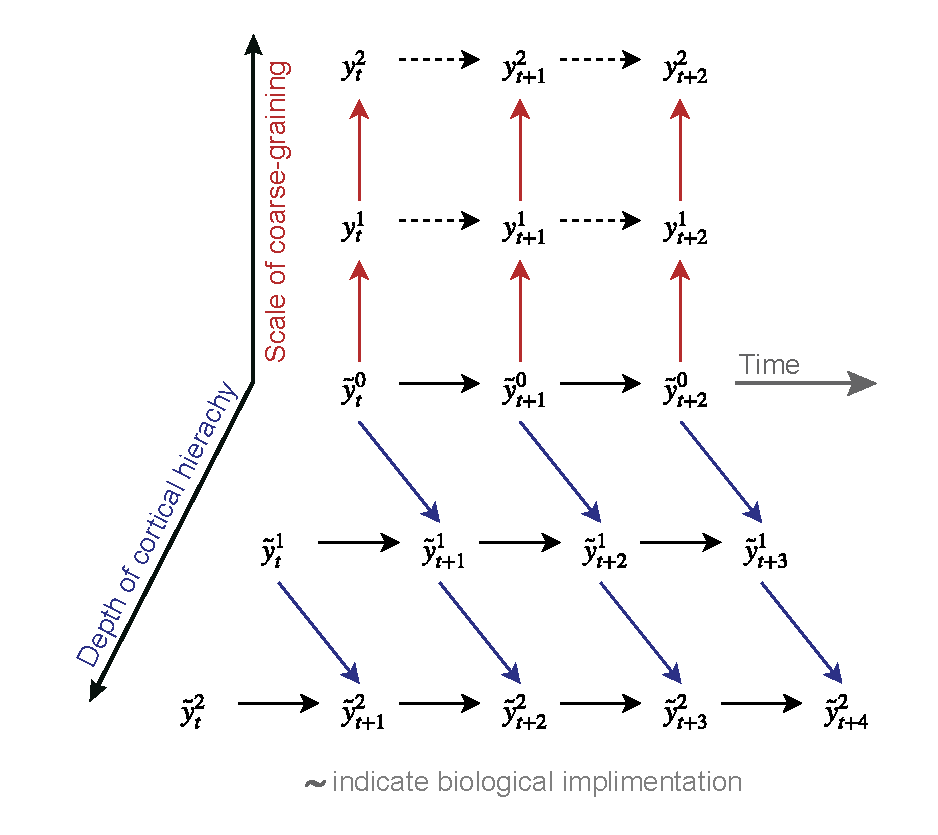
\includegraphics[width=\textwidth]{WritingMaterials/SeperationOfCGandCortHierachy.pdf}
				\label{fig:hierarchy}
			\end{figure}


            \begin{WritingMaterials}
    			@ Of course, from evolutionary perspective, neural system should develop a better hardware to support neural coarse-graining

				@ For example, pooling layers in CNN is an implementation of coarse-graining function. It' is very plausible visual processing hierarchy in the neural system realises pooling layers.


				@ It is possible that the neural system represents higher-level information processing by low level physical subtract. For example, studies have found representation for summery statistics of signal and neural. population.\needref{neural representation for summery statistics}\\
				From this point of view, sensory hierarchy may extend along with levels of coarse-graining.
            \end{WritingMaterials}
        

        
               
\rlend

\rlstart{2}	
        \subsection{Dynamical Boundary}
        Our theory predicts that the physical boundary of a conscious system is dynamical. The boundary is determined by elements forming high NTIC. This implies that when the structure of interaction between elements changes the physical boundaries support consciousness should also change. If some coarse-grained variables encode environmental information, they may become necessary components to form high NTIC. In such case, these coarse-grained variables are "recruited" inside the boundary of conscious processes. Note that, due to synergetic information, even recruiting some new variables may largely increase the level of NTIC. 
        This may explain why consciousness is tightly associated with binding and integration of information in human perception and cognition. Another crucial implication is that the same neural substrates may not be always involved in conscious processing rather it depends on whether it creates high NTIC with other members in the neural system. \needfig{Maybe I need a figure h  ere as well}
    
\rlend